\documentclass[twocolumn,10pt]{article}

\usepackage[a4paper,hmargin=1.5cm,vmargin=2.5cm,]{geometry}
\setlength{\columnsep}{0.7cm}
\usepackage{palatino}
\usepackage{graphicx}
\usepackage[utf8]{inputenc}
\usepackage{hyperref}
\urlstyle{same} % no tt font for URLs

\usepackage{natbib}
\bibliographystyle{genome_research}
%\setcitestyle{aysep={}} 

\usepackage[dvipsnames]{xcolor}
\hypersetup{
    colorlinks,
    linkcolor={blue!50!black},
    citecolor={blue!50!black},
    urlcolor={blue!50!black}
}
\renewcommand{\dbltopfraction}{0.7}
\renewcommand{\textfraction}{0.2}

\begin{document}

\setcounter{secnumdepth}{0}

\twocolumn[{%
\centering
\textbf{\Large Analysing single-cell bisulfite sequencing data with scbs}
\vspace{1.5ex}

Lukas P. M. Kremer, Leonie Küchenhoff, ..., Simon Anders\\
{\footnotesize University of Heidelberg, Germany}
\vspace{1.5ex}

November 2021
\vspace{6ex}
}]

\section{Abstract}

[...]

\section{Introduction}

Sequencing-based assays with single-cell resolution have offered new means to understand the differences between the cells making up a sample. Single-cell RNA sequencing techniques have matured at great pace in recent years, and methods to study chromatin are rapidly catching up. Of special interest here is DNA methylation, i.e., the methylation of bases in the DNA, because DNA methylation patterns are passed on to daughter cells in cell division. Especially in mammals, such methylation chiefly occurs at cytosine bases that are immediately after followed by guanine bases, so-called CpG sites. 

To detect CpG methylation by sequencing, bisulfite conversion is commonly employed: treatment of DNA with bisulfite causes unmethylated guanine bases to be deaminated to uracil, which is paired with thymine in subsequent PCR. Therefore, unmethylated CpGs are read as TG in sequencing of bisulfite-converted DNA while only methylated CpG is correctly read as CG \citep{Frommer_1992}. Such so-called bisulfite sequencing has been used for bulk samples since long, and methods for bisulfite sequencing with single-cell resolution \citep{Smallwood_2014} have become commercially available recently and are increasingly used.

CpG dinocleotides are underrepresented in eukariotic genomes (due to their vulnerability to mutation by conversion to TpG due to accidental deanimation), and the majority of existing CpG sites are methylated. Presence or absence of the methyl group at CpG sites is believed to have effect on gene regulation, with methylation inhibiting transcription. Methylating DNA during differentiation is therefore conjectured to be an important mechanism to silence genome regions that are not needed in the target lineage. One important application of single-cell bisulfite sequencing (sc-BS-Seq) therefore lies in the study of differentiation processes.

In the present paper, we discuss strategies to analyse sc-BS-Seq data, suggest improvement to current approaches, show their value in a benchmark, and present software to perform the improved analysis methods.

\subsection{Standard approach}

We start by briefly reviewing the standard approach of analysing single-cell \emph{RNA}-Seq data, and how this approach is typically adapted to the case of DNA methylation data.

The starting point in scRNA-Seq is a matrix of UMI counts (i.e. of counts of distinct RNA molecules), one row for each cell and one column for each gene. As a first step towards assigning cell types or states to cells, one needs to establish which cells are similar to each other, and to this end, find a way to quantify the distance (i.e., dissimilarity) between any two given cells' transcriptional profile. A standard approach, used with minor variation in virtually all recent research and automated by popular software such as Seurat or ScanPy, is as follows: One first accounts for cell-to-cell variation in sequencing depth by dividing each UMI count by the respective cell's total UMI count, then transforms to a homoskedastic scale by taking the logarithm. In order to avoid matrix elements with zero count to be transformed to minus infinity, one typically adds a very small ``pseudocount'' (often $10^{-5}$) to the normalized fractions before taking the logarithm. Now, one could use Euclidean distances of these vectors  of logarithmized fractions as dissimilarity score. However, these scores would be exceedingly noisy due to the strong Poisson noise introduced by the many genes with very low counts. Therefore, one performs a principal component analysis (PCA), keeping only the top few (typically, 20 to 50) components. As Poisson noise is uncorrelated between genes, it will average out in the top principal components. Therefore, Euclidean distances between these "PCA space" vectors provide a robust dissimilarity score, which can subsequently be used as input to methods like t-SNE and UMAP, which provide a two-dimensional representation of the data. The PCA space representation is furthermore used for clustering (assigning cells to groups by similarity) and trajectory finding (identifying elongated manifolds in PCA space and assigning cells to quasi-1D positions along them).

This procedure is commonly adapted when working with single-cell DNA-methylation data, so that all the tools used in scRNA-Seq downstream of the PCA step can be used. The question is therefore how to construct a suitable matrix as input for the PCA. A simple and popular approach is to tile the genome into windows of, say, 100 kB size, and calculate for each cell the average methylation of the DNA within each window. To this end, we identify all CpG sites in the window for which we have coverage with at least one read and can hence call the CpG to be either unmethylated or methylated in the cell. Then we denote as average DNA methylation of this window in a given cell the proportion of observed CpG sites in the window have been found to be methylated. This yields a matrix, with one row for each cell and one column for each window from the genome tiling, comprising numbers (methylation fractions) between 0 and 1. This matrix is now subjected to PCA.

As an example, we will us in this paper data from XX et al., who have performed sc-BS on [...] and analysed their data in the manner just described. Figure 1a shows a UMAP plot, derived from our re-analysis of the data, using a tiling of the genome into windows of size 100 kb. As one can see, the approach is suitable to see clear structure in the data, observe ...

Nevertheless, this analysis strategy has substantial room for improvement, as we will discuss next. Here, we discuss the proposed improvements only qualitatively. For the mathematical details, please see the Methods section. 

\begin{figure}
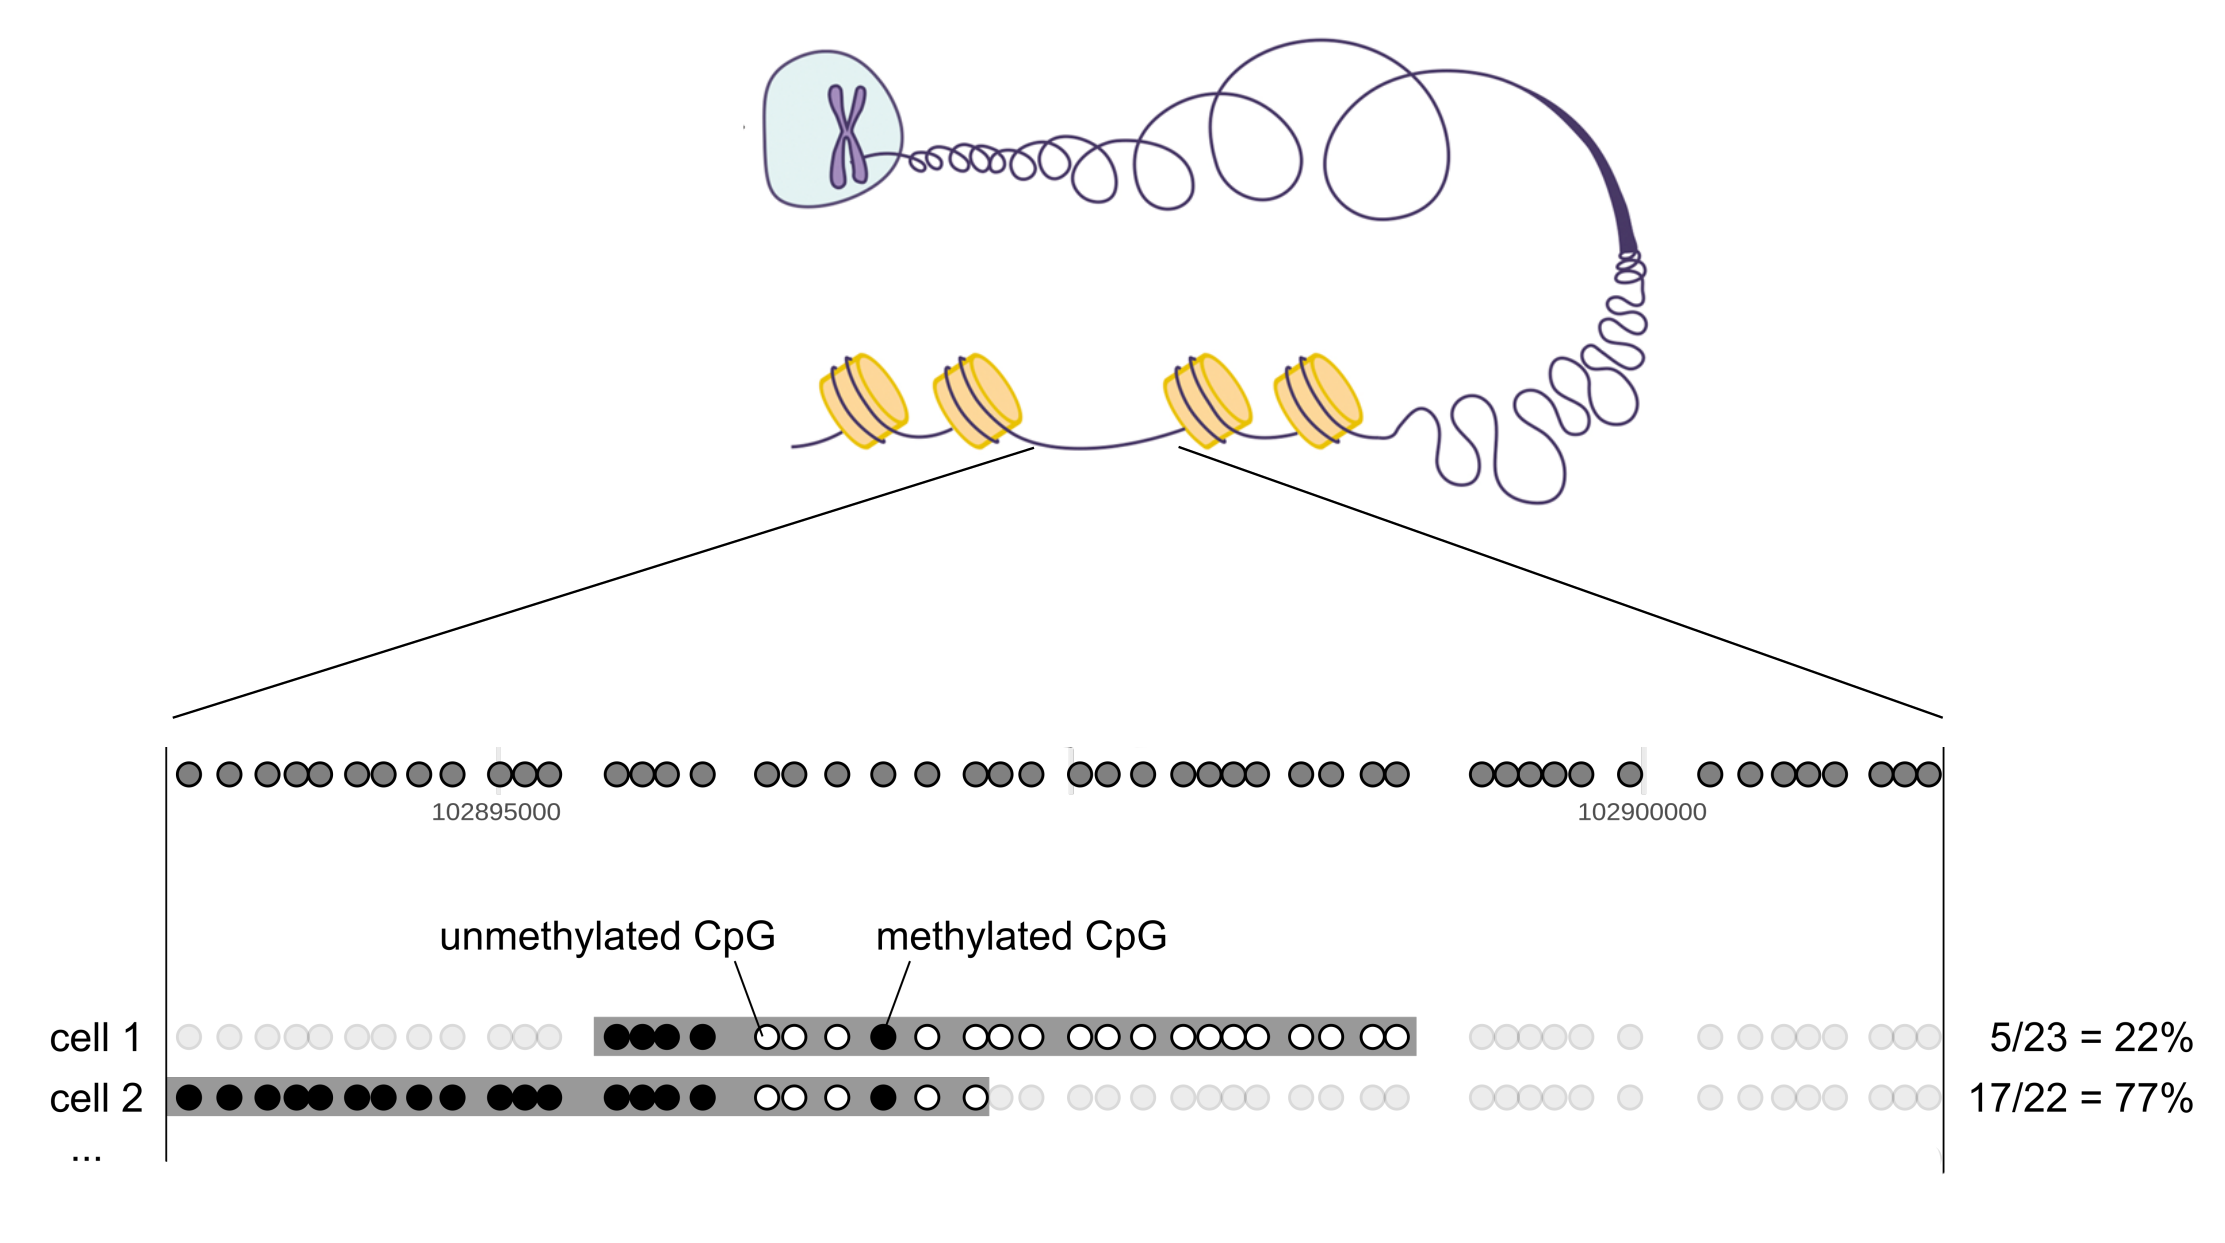
\includegraphics[width=\columnwidth]{need_for_relative_meth.png}
\caption{\textbf{Effect of read position:} Depicted is a genomic interval along a chromosome, for which DNA methylation is to be quantified. Two cells cover differing parts of the interval with one read each. If one simply counts for each cell which fraction of the covered CpG sites are methylated, one obtains very different values for the two cells.}
\end{figure}

\section{Three improvements to processing scBS data}

\subsection{Smoothing residuals}

We first discuss the task of quantifying the level of methylation in given, fixed, genomic interval. In Figure \ref{}, such an interval is covered by a single read for each of the two cells shown. The read from the cell 2 shows much more methylation than the read from cell 1, and a simple analysis would therefore consider that cell as having stronger methylation in the interval. However, given that the two reads agree wherever they overlap, a more parsimonous interpretation would be that the cells do not show difference in methylation within the interval. Rather, both cells, and similarly maybe most other cells, might have stronger methylation in the left third of the interval than in the middle one.

Therefore, we propose to not first obtain, for each CpG position, an average methylation across all cells and, then quantify for each individual cell its deviation from this average. In Figure \ref{}, the curved line depicts such an average over all cells, the red vertical lines show an individual cell's deviation from the ensemble average. We take the lengths of the red lines as signed values (``redidual''), positive for lines extending upwards from the curve (methylated CpG) and negative for lines extending downwards (unmethylated CpG), and take the average over the residual for all the CpGs in the interval that are covered by reads from this cell. The value thus obtained is what we use to quantify this cell's (relative) methylation in the interval. For a genome tiled into such intervals, we thus obtain a matrix, one row per interval, one column per cell, that can be used for downstream analysis, e.g., as input for a PCA.

The signal to noise ratio in a matrix thus obtained will be much better than in a matrix obtained by simply averaging absolute methylation (0 or 1) over all the cell's covered CpG in a region. The reason for this is that we reduce the variation in situation as the one depicted in FIgure \ref{}, where absolute methylation might differ strongly even though there is no actual evidence for a difference between the two cells.

How should one obtain the ensemble average (the curved line in Fig.\ \ref{})? A simple approach to get a value for a spcific CpG would be to take all cells with read coverage for the CpG and use the fraction of these that show the CpG as methylated. However, especially when only few cells offer coverage, these averages will be very noisy. Therefore, we propose to smoothen using a kernel smoother, i.e., by performing a kernel-weighted average over the CpG site's neighborhood. The kernel bandwidth (i.e., the size of the neighborhood to average over) is a tuning parameter; we got good results with XXX bp and used this value for the examples presented here.

\subsection{PCA with imputation}

The standard PCA algorithm cannot deal with missing data. Therefore, one would need to make intervals wide enough to ensure that every interval is covered by at least one read for most windows and discard any interval that is not covered by any single cell. Hence, a naive analysis has to resort to a coarse tiling of the genome. To counter this, we propose a simple and straightforward way to deal with missing data in the input matrix to a PCA: In a first iteration, we replace each missing value in the centered input matrix with zero, then run the PCA. Then, these zeroes are replaced by the value predicted by the PCA and the PCA is rerun. Convergence is typically achieved after two to four iterations. For details, see Methods. 

The possibility to perform PCA with missing data allows us to use a shorter and thus more intervals and hence provide the PCA with richer input data.

\subsection{Finding variably methylated regions}

Typically, some regions in a chromosome will have very similar methylation status in all cells (most commonly, fully methylated in nearly all cells) while other regions show variability in methylation across cells. Only the latter regions are of value for our goal of quantitating dissimilarity between cells. We call these the variably methylated regions (VMRs).

So far, we have discussed dividing up (tiling) each chromosme genome into non-overlapping, equal-sized intervals, and quantitating the methylation of each such window. Such rigid placing of interval boundaries is unlikely to be optimal: for example, a VMR might be much smaller than a tile and its signal will hence be drowned out by the larger part of uninformative CpGs that are equal in all cells, when averaging over all the CpG sites in the tile.

Therefore, we propose the folloing approach: Divide up the chromosome into many \emph{overlapping} windows, that start at regular multiples of a fixed, small, step size. Quantify the methylation of each cell in each window by averaging the cell's methylation residuals over all CpGs in the window, as described above and depicted in Figure\ \ref{}. Then, calculate for each window the variance of these values over all cells. Select, say, the top XX\% windows with the highest variances and mark them as VMRs. Wherever thus marked windows overlap or are divided by only a small gap, merge them into one larger VMR. Then, calculate for each of these laregr VMRs the methylation signal, as before, by averaging for each cell over the residuals of all contained CpGs.

In this manner, we obtain a methylation matrix, with one column per cell and one row per VMR, that is, in a sense, richer in information and has better signal-to-noise ratio than the matrix obtained by the simple analysis sketched at the very beginning. As we demonstrate below, a PCA performed on such a matrix provided a distance metric for the cells that contains more information on biological detail than one from a simpler analysis. 

Besides providing better input for the distance calculations, the identified VMRs can also be compared with genomic annotation, thus providing a useful starting point for examining the data with methods from functional genomics.

\section{The scbs Python package}

We have implemented the approach just described in a Python package, called ``scbs'', that offers the following functionality: ...

The code is open source, the source-code and the package are available from ..., where detailled documentation on usage is provided as well.

\section{Comparison}

Now, we can compare the simple analysis described initially with an analysis using our method, in order to demonstrate that it improves results.

\section{Discussion and Conclusion}

...

\end{document}